\section{Problem 1}
\subsection{Prolem 1(a)}
\aay{\Cref{fig:dualq1} shows equivalent configuration of the primal given in the problem statement in the dual plane. }

\begin{figure}[H]
	\centering{
		\resizebox{!}{6cm}{
			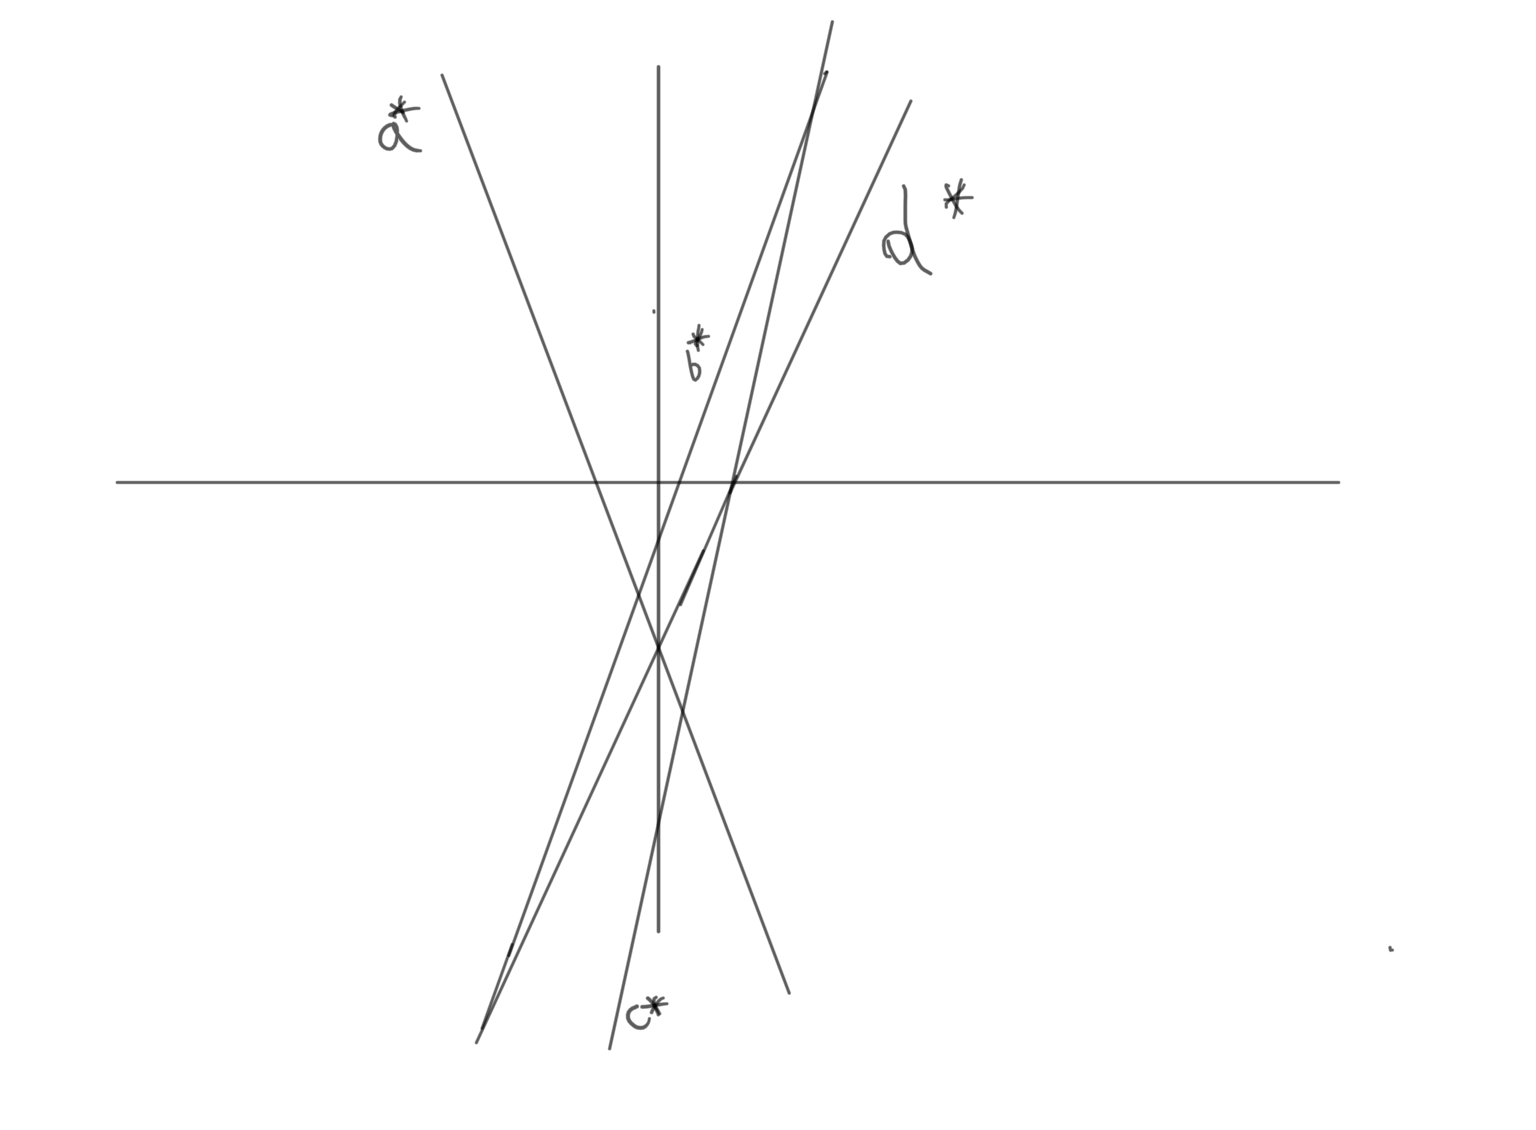
\includegraphics[scale=.1]{Images/5a.png}
		
		}
	} 
	\caption{(a) Dual of the given figure. \aay{Dual of an object in primal is named with an additional asterisk (*) in the dual representation.} } 
	\label{fig:dualq1}
\end{figure}


\subsection{Problem 1(b)}
\subsubsection{General Case}
We propose a \textbf{branch and merge} algorithm for the problem. Intuitively, we exploit the nature of dual transformation of individual line segments, obtain potential regions where the new point (corresponding to the stabber) can lie for each line and then find an intersection of these potential regions of all line segments using a branch and merge technique. 


To begin with we consider all the general \textbf{assumptions} that no line is vertical (otherwise we will have an empty region between the duals of end of this line segment). In order to avoid this we can possible tilt the line a bit and to not disrupt the overall relative arrangement and tilt it back once the solution is obtained. (Other way of dealing with vertical lines can be rotating the whole plane along). 

Now we consider the lines $lp1, lp2$ in dual plane obtained by dual of ends $p1, p2$ of a line segment $l$ in original plane. From our initial assumption we know that the $lp1$ and $lp2$ are not parallel. Also we know that any line intersecting line segment $l$ must be concurrent with $lp1$ and $lp2$. Moreover, we cannot have a vertical line segment in the dual plane (as that would render a point with infinte y-coordinate in the primal subplane). The region between the two intersecting lines $lp1,\ lp2$ can be seen as 4 unequal quadrants or wedges (not necessarily rectilinear). We define two such quadrants as \textbf{double wedge} formed by the primal points $lp1, lp2$.  This gives us the following lemma:

\begin{lemma} \label{lem:two}
 Any line $s$ intersects a line segment $l$ with endpoints $p1$, $p2$ iff the point the dual point corresponding to $s$ i.e. $p_s$ lies in the double wedge of $lp1,\ lp2$.
\end{lemma}

\Cref{lem:two} intuitively solves the entire problem as the intersection of double wedges of all the line segments is the region which contains dual points corresponding to all the stabbers in primal. If this intersection is empty, we claim that a stabber to line segments in primal plane doesn't exist. Otherwise, we can pick any point from this region and the corresponding line should clearly be a feasible stabber in the primal plane.

Formally, we now employ a branch and merge approach to divide the line segments into two almost equal partitions and obtain the intersection of double wedges of all the lines in two halfs recursively, and as a final step merge the two regions in $O(n)$ time. Lets call the regions obtained as a result of intersection of double wedges of given line segments in the dual plane as \textbf{stabbing region} (the term is correct as every point in this stabbing region refers to a stabber in the corresponding primal plane).

Now what we are left with is formulating the merge step where we merge the stabbing regions of the two partitions. Since the stabbing regions are nothing but a set of polygons (in the dual plane), we can use the plane sweep technique (as discussed in lectures) and find the intersection of the two stabbing regions (polygons) in time $O(v_1+v_2)$ where $v_1$, $v_2$ are the number of vertices in the two stabbing regions (polygons) respectively. 

We now bound number of vertices is by
$n_1$ (respectively $n_2$), which are the number of line segments used to in the initial partition, as given by the following lemma : 
\begin{lemma}
$v$ i.e. the number of vertices of a stabbing region obtained by intersection of double wedges corresponding to $n$ line segments, is $O(n)$
\end{lemma}
\begin{proof}
Clearly every double wedge creates amost 4 new edges (more specifically half edges) which is $O(1)$. Furthermore, number of polygons that may arise in a stabbing region of $n$ line segments is atmost $n+1$. Now each we can have $4$ different types of edges depending on the relative arrangement on a double wedge. For each type of edge, we can have atmost $2n+1$ edges as part of the $n+1$ (at most) polygons. This leaves us with at most $8n+4$ edges and thus $O(n) $ vertices defining the stabbing region.
\end{proof}

This completes the formulation of algorithm, we can now merge the two half in time $O(v_1+v_2) = O(n_1+n_2)$ using a simple plane sweep algorithm (as discussed in lectures). Overal time complexity is given by :
\begin{align*}
     T(n) &= T(n_1)+T(n_2)+O(n_1+n_2) \\
    \implies  T(n) &= T(\frac{n}{2}) + T(\frac{n}{2}) + O(n)\\
    \implies T(n) &= O(nlogn)
\end{align*}

If the computed region is empty then we can directly claim that the instance is a NO instance as no stabber exists.

We also point out that a rather naive approach would have been considering finding the intersection of stabbing regions one by one for each double wedge. This would have given us an $O(n^2)$ runtime algorithms, but instead merge and branch improved upon this approach by giving an algorithm running in \textbf{time} $\bm{O(nlogn)}$.


\subsubsection{Horizontal lines}
Now we consider the problem of deciding whether there exists any stabber of given set of \emph{horizontal} line segments. (In fact this approach can easily be used for any pair of parallel line segments by a simple rotation of axis).

Intuitively, we consider the given horizontal intervals as buckets acting as constraints for the stabber and we \textbf{guess over the possible tilts} (towards both directions from the vertical) for the stabber confined in these buckets. We slack a bit and use a simple LP formulation to solve this problem as the fatigue accumulated by the end of the semester, resists us from thinking about any other beautiful geometric-algorithms.

Formally, we write a \textbf{2D linear program} with the two variables as $m_{stab},\ c_{stab}$. These correspond to the equation $y=m_{stab}x+c_{stab}$ of the stabbing line. Consider the input line segments $\{l_i\ |\ \forall i \in [n]\}$ as a set of pairs of end points $\{(p^1_i, p^2_i)\ | \ \forall i\in [n]\}$, each point $p$ is represented by its coordinates as $(x_p, y_p)$. We consider that the given tuple $(p^1_i, p^2_i)$ is such that $x_{p^1_i}\leq x_{p^2_i}$, i.e. the points are arranged in increasing order of x-coordinates. The required linear programs are defined as follows:

\begin{equation*}
\begin{array}{ll@{}ll}
\text{maximize}  &  m_{stab} &\\
\text{subject to}& m_{stab}\ x^1_i + c_{stab}\geq y_i &\forall i \in [n]\\
    & m_{stab}\ x^2_i  + c_{stab} \leq y_i &\forall i \in [n]\\
    & m\leq 0
\end{array}
\end{equation*}


\begin{equation*}
\begin{array}{ll@{}ll}
\text{minimize}  &  m_{stab} &\\
\text{subject to}& m_{stab}\ x^1_i + c_{stab}\leq y_i &\forall i \in [n]\\
    & m_{stab}\ x^2_i  + c_{stab} \geq y_i &\forall i \in [n]\\
    & m\geq 0
\end{array}
\end{equation*}

The above two linear programs work independently searching for a stabbing line with negative and positive slopes respectively.  If none of the above LPs return a feasible solution, we directly output that the input instance is a NO instance. It should be noted that the LP does not return any feasible solution, it is indeed returns the stabbing line with aligning closest to the horizontal i.e. the \textbf{lowest laying stabber}. From the work \cite{megiddo1984linear} by Nimrod Megiddo of Tel Aviv University, we know that the linear programming problem in $d$ variables and $n_c$ constraints can
be solved in $O(n_c)$ time given d is fixed/constant. (This bound actually follows from a multidimensional search technique, for more depth into this we refer to \cite{megiddo1984linear}). Both linear programs proposed by us have $d=2$ and $n_c =O(n)$, thereby giving a complexity $\bm{O(n)}$ \textbf{time and space.}

